%-*-coding: utf-8-*-

\chapter{Эксперименты и результаты}

\section{Решаемые задачи}
В данном разделе будут описаны задачи, на которых будет проверяться качество предложенной модели.
\vspace{5mm}

\noindent \textbf{Задача классификации эмоционального тона предложения}\par
Задача классификации эмоционального тона предложения состоит в оценке эмоциональной характеристики предложения. В данной главе будут рассмотрены наборы данных, которые содержат обзоры фильмов. 
Предложенная модель должна будет предсказать, какому из пяти эмоциоанльных классов относится обзор:
\emph{очень негативный}, \emph{негативный}, \emph{нейтральный}, \emph{позитивный}, \emph{очень позитивный}.
\vspace{5mm}

\noindent \textbf{Задача классификации вопросов}\par
Задача классификации вопросов состоит в определении к какому типу принадлежит вопрос:
аббревиатура, сущность (животное, еда и т.д), описательный, личность, расположение, числовой.
\vspace{5mm}

\noindent \textbf{Задача классификации субъективных и объективных предложений}\par
Задача классификации субъективных и объективных предложений состоит в определении, является ли данное предложение объективным или субъективным. То есть является задачей бинарной классификации.

\section{Описание наборов данных и методики тестирования}
Предложенное решение было протестировано на нескольких наборах данных. 
Они содержат синтаксические деревья либо предложения. 
Для предложений были построены синтаскические деревья с помощью[ссылка].
\vspace{5mm}

\noindent \begin{minipage}{\linewidth}
\captionof{table}{\textbf{Наборы данных}} \label{tab:title} 
\begin{tabular}{|c|c|c|c|c|}
\hline
\multirow{2}{*}
  {Название}      & Кол-во         & Средняя длина          & Кол-во          & Кол-во  \\
                  & классов        & предложения            & трен. примеров  & тест. примеров \\ \hline
\textbf{SST-1}    & 5              & 18                     &  11855          &  2210    \\ \hline
\textbf{MR}       & 2              & 20                     &  10662          &  CV-5    \\ \hline
\textbf{Subj}     & 2              & 23                     &  10000          &  CV-5     \\ \hline
\textbf{TREC}     & 6              & 10                     &  5952           &  500    \\ \hline
\end{tabular}
\vspace{5mm}
\end{minipage}

\begin{itemize}
\item{\textbf{SST-1}}~--- набор данных с обзорами фильмов, содержит синтаксические деревья разбора\\
\item{\textbf{MR}}~--- набор данных с обзорами фильмов, содержит предложения\\
\item{\textbf{Subj}}~--- набор данных с субъективными и объективными утверждениями, содержит предложения\\
\item{\textbf{TREC}}~--- набор данных с шестью типами вопросов, содержит предложения
\end{itemize}
\vspace{5mm}

CV-5 в последнем столбце означает, что тестирование на наборе будет проведено с использованием техники скользящего контроля с параметром $K=5$

Для обучения был использован язык Python 3.4 и фреймворк символьных вычислений Tensorflow[ссылка].
Обучение проводилось с помощью оптимизаторов Adam[ссылка] и Adagrad[ссылка].

В процессе обучения архитектур была использована $L_2$ регуляризация[ссылка].
Это подход, когда к минимизируемой ошибке добавляются квадраты всех параметров сети, умноженных на некоторый коэффициент.
Он предотвращает переобучение параметров, так как параметры не могут принимать большие значения из-за увеличения ошибки.
$L_2$ регуляризация задается коэффициентом регуляризации $\lambda$.

Кроме того, использовался dropout (дропаут)[ссылка]. 
Эта техника заключается в том, что во время обучения некоторые нейроны с некоторой вероятностью не участвуют в предсказании.
Этот подход предотвращает cоадоптацию нейронов. Он задается вероятностью участия нейрона в предсказании $p$.

Обучение происходило минибатчами. Один минибатч включает в себя несколько тренировочных примеров, ошибка и градиент оптимизатора
берется как среднее ошибок и среднее градиентов по примерам в минибатче. Это сделано для более плавного роста ROC прямой и, следовательно, более быстрой сходимости. Размер минибатча составлял 25.

В наборе данных \textbf{SST-1} проаннатированы все поддеревья, 
поэтому для увеличения эффективности обучения ошибка учитывается не только от корня дерева, но и от всех поддеревьев.

\subsection{Тестирование архитектуры с локальными контекстами}
В данном разделе мы рассмотрим эксперименты над архитектурами, с вычислением локальных контекстов.

Сначала рассмотрим использование простой рекурсивной модели в качестве механизма пересчета поддеревьев.
Классификация происходит с помощью полносвязного слоя, как это было описано в конце раздела 2.2.5.

\vspace{5mm}
\noindent \begin{minipage}{\linewidth}
\captionof{table}{\textbf{Вычисление локальных контекстов на основе CNN}} \label{tab:title} 
\begin{tabular}{|c|c|c|c|c|c|c|}
\hline
\multirow{2}{*}{Набор} &                \multicolumn{6}{c|}{Размер k-граммы} \\ \cline{2-7} 
     данных            & \textbf{-} & \textbf{2} & \textbf{3} & \textbf{4} & \textbf{5} & \textbf{2-5} \\ \hline
\textbf{SST-1}         & 45.5\%     & 46.7\%     & 46.3\%     & 46.1\%     &  46.1\%    & \textbf{47.2}\% \\ \hline
\textbf{MR}            & 75.5\%     & 77.4\%     & 77.0\%     & 76.5\%     &  76.6\%    & \textbf{77.6}\%  \\ \hline
\textbf{Subj}          & 88.8\%     & 90.9\%     & 90.8\%     & 90.9\%     &  90.5\%    & \textbf{91.1}\% \\ \hline
\textbf{TREC}          & 89.2\%     & 89.9\%     & \textbf{91.5}\%     & 91.1\%     &  90.9\%    & 90.3\% \\ \hline
\end{tabular}
\end{minipage}
\vspace{5mm}

\noindent \begin{minipage}{\linewidth}
\captionof{table}{\textbf{Вычисление локальных контекстов на основе LSTM}} \label{tab:title} 
\begin{tabular}{|c|c|c|c|c|c|c|}
\hline
\multirow{2}{*}{Набор}   &         \multicolumn{6}{c|}{Размер k-граммы} \\ \cline{2-7} 
     данных              & \textbf{-} & \textbf{2} & \textbf{3} & \textbf{4} & \textbf{5} & \textbf{2-5} \\ \hline
\textbf{SST-1}           &  45.5\%    & 46.4\%     &\textbf{46.4}\%& 46.3\%     &  46.2\%    & 46.2\%           \\  \hline
\textbf{MR}              &  75.5\%    & 76.3\%     & 76.2\%     & 76.3\%     & 76.1\%     & \textbf{76.4}\% \\ \hline
\textbf{Subj}            &  88.8\%    & 89.3\%     & 89.3\%     & 89.6\%     &\textbf{89.8}\%    & 89.7\% \\ \hline
\textbf{TREC}            &  89.2\%    & 84.9\%     & \textbf{87.1}\%     & 87.1\%     &  86.9\%    & 88.6\%  \\ \hline
\end{tabular}
\vspace{5mm}
\end{minipage}
\vspace{5mm}

Первый столбец описывает модель без использования локальных контекстов, то есть в качестве векторного представления локального контекста слова выступает векторное представление слова.

Последний столбец описывает модель, которая считает векторное представление $k$-грамм для $k=2,3,4,5$ и конкатенирует их.

В общем и целом подход вычисления локального контекста превосходит на всех наборах данных базовую модель РНТС[статья], которая использует простой рекурсивный подсчет поддеревьев.

Мы можем видеть, что для каждой задачи, лучший результат достигается при разных значениях $k$. В каких-то задачах достаточно учитывать рядом стоящее слово, в других~--- несколько слов.

Но вне зависимости от задачи, можно пронаблюдать закономерность, что 
вычисление длинных $k$-грамм (при $k=5$) не приводит к хорошему результату, 
так как в контекст начинают попадать далекие слова, 
которые могут иметь достаточно произвольный характер относительно первого слова.

Мы видим, что использование LSTM в качестве механизма захвата контекста значительно проигрывает CNN.
Это можно объяснить тем, что важен только сам набор слов, но не их порядок. 
CNN больше подходит для данной задачи, в основе же LSTM лежит последовательная обработка слов, то есть ей важен порядок слов.

Вычисление на основе CNN обучается достаточно быстро, но склонно к переобучению, поэтому требует кропотливой подборки гиперпараметров, таких как количество карт признаков, а также $\lambda$ и $p$.

\begin{figure}[H]
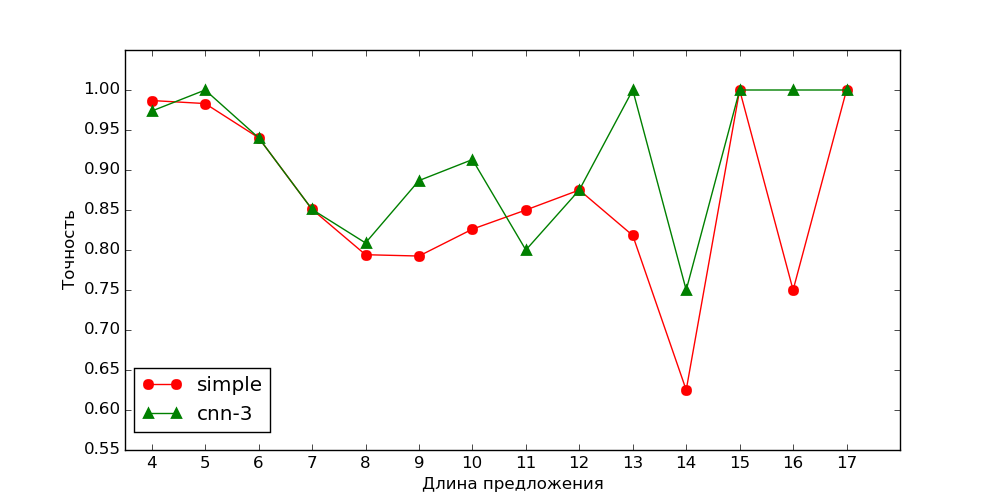
\includegraphics[scale=0.75]{trec_comp}
\caption{\textbf{Зависимость точности предсказания от длины предложения на TREC}}
\label{fig:context_ex}
\end{figure}
На данном графике сравниваются модели \textbf{CNN-3} и модель без использования локальных контекстов на наборе данных \textbf{TREC}. Точность здесь равна отношению правильно классифицированных предложений заданой длины к общему количеству предложений этой длины. 

Можно видеть, что обе модели хорошо справляются с короткими предложениями, длина которых от $4$ до $8$.
Но модель \textbf{CNN-3} лучше справляется с более длинными предложениями.

Аналогичное можно наблюдать и на наборе данных \textbf{SUBJ}.

\begin{figure}[H]
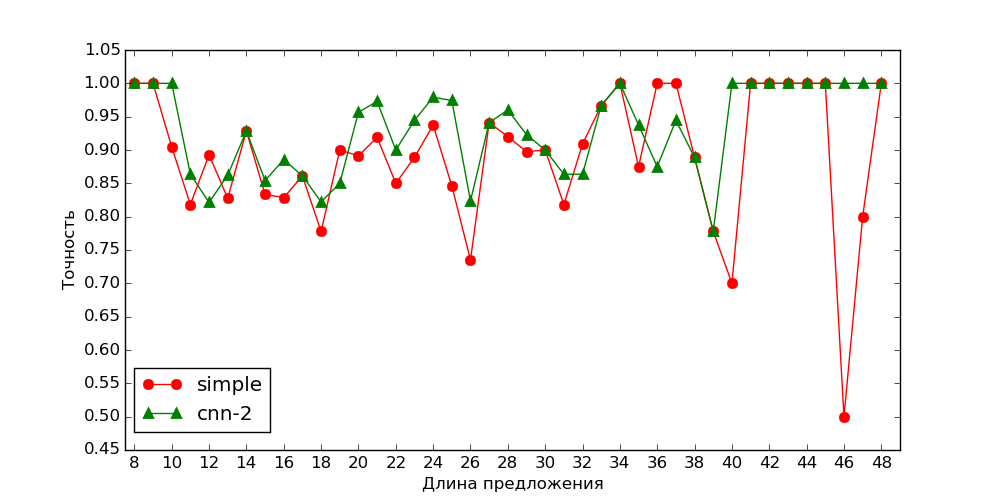
\includegraphics[scale=0.75]{subj_comp}
\caption{\textbf{Зависимость точности предсказания от длины предложения на Subj}}
\label{fig:context_ex}
\end{figure}

Теперь рассмотрим  древовидный LSTM (TreeLSTM) в качестве механизма пересчета поддеревьев, 
чтобы показать, что захват локальных контекстов работает не только на одном методе, 
но может применяться и к более продвинутым моделям.

\vspace{5mm}
\noindent \begin{minipage}{\linewidth}
\captionof{table}{\textbf{Результаты TreeLSTM c контекстами CNN}} \label{tab:title} 
\begin{tabular}{|c|c|c|c|c|c|c|}
\hline
\multirow{2}{*}{Набор}   &                \multicolumn{6}{c|}{Размер k-граммы} \\ \cline{2-7} 
     данных              & \textbf{-} & \textbf{2} & \textbf{3} & \textbf{4} & \textbf{5} & \textbf{2-5} \\ \hline
\textbf{SST-1}           &            &            &            &            &            &        \\ \hline
\textbf{MR}              & 77.5\%     &  79.6\%    & 79.0\%     & 78.8\%     & 78.7\%     & \textbf{79.7}\% \\\hline
\textbf{Subj}            & 90.7\%     &  90.3\%    & 91.3\%     & \textbf{91.4}\%     & 91.0\%     &  91.2\% \\\hline
\textbf{TREC}            & 90.7\%     &  \textbf{92.5}\%    & 92.1\%     & 91.8\%     & 91.7\%     &  91.6\% \\\hline
\end{tabular}
\end{minipage}
\vspace{5mm}

Здесь мы также можем видеть улучшение результатов при вычислении локальных контекстов.

\subsection{Тестирование архитектур со значимыми поддеревьями}

Напомним, что в подходе со значимыми поддеревьями, количество значимых поддеревьев определяется функцией $K$.

К сожалению, в ранмках Tensorflow сделать $K$ функцией не удалось, поэтому будут рассмотрены только постоянные значения $K$.

\vspace{5mm}
\noindent \begin{minipage}{\linewidth}
\captionof{table}{\textbf{Архитектуры с TopK пересчетом поддеревьев}} \label{tab:title} 
\begin{tabular}{|c|c|c|c|c|c|}
\hline
\multirow{2}{*}{Набор}   &  \multicolumn{4}{c|}{Значения K} \\ \cline{2-5} 
     данных              &  \textbf{2}  & \textbf{4}   & \textbf{6} & \textbf{8} \\ \hline
\textbf{SST-1}           & 43.0\%       &  44.7\% & \textbf{45.0}\% & 44.9\%     \\ \hline
\textbf{MR}              & 71.3\%       & 73.8\%  & \textbf{74.7}\% & 74.1\%     \\ \hline
\textbf{Subj}            & 83.5\%       & 85.3\%       & 86.1\%     & \textbf{87.0}\% \\ \hline
\textbf{TREC}            & 85.0\%       & 86.7\% & \textbf{86.8}\%     & 86.3\%     \\ \hline
\end{tabular}
\end{minipage}
\vspace{5mm}

Примечательным моментом является то, что на наборе данных \textbf{TREC}, результат при $K=4$ близок к наилучшему, а на остальных наборах данных лучший результат достигается при большем значении $K$.
Это происходит потому, что средняя длина предложений остальных наборов значительно больше, чем в \textbf{TREC}.

Можно видеть, что данный подход имеет право на жизнь, но результаты оставляют желать лучшего.
Потенциал \textquote{значимых поддеревьев} будет раскрыт в следующем разделе.

\subsection{Архитектуры с наилучшими результатами}

В данном разделе будут рассмотрены архитектуры, показавшие хорошие результаты на некоторых наборах данных.

\vspace{5mm}
\noindent \begin{minipage}{\linewidth}
\captionof{table}{\textbf{Мда}} \label{tab:title} 
\begin{tabular}{|c|c|c|c|c|c|}
\hline
\multirow{2}{*}{Набор}   &             \multicolumn{5}{c|}{Архитектуры} \\ \cline{2-6} 
     данных              &  \textbf{A}  & \textbf{B} & \textbf{C} & \textbf{D} & \textbf{E} \\ \hline
\textbf{SST-1}           & 48.7\%       & 48.6\%     & 48.8\%     &            &            \\ \hline
\textbf{MR}              & 79.0\%       & 79.6\%     &            &            &            \\ \hline
\textbf{Subj}            & 91.5\%       & 91.2\%     & 91.4\%     & 90.0\%     & 91.4\%     \\ \hline
\textbf{TREC}            & 93.1\%       & 92.7\%     &            & 91.6-93.6\%& 91.7\%           \\ \hline
\end{tabular}
\end{minipage}
\vspace{5mm}

Архитектура \textbf{A}~--- локальный контекст считается \textbf{CNN-2}, в качестве механизма пересчета поддеревьев используется древовидная LSTM. После подсчета векторного представления $f_v$ поддерева вершины $v$ считается LSTM от слов поддерева, в которую помимо слов из поддерева подается $f_v$. То есть $f_v$ служит вспомогательным вектором для
LSTM. После чего пара из $(f_v, LSTM(v))$ подается в полносвязный классификатор.

Архитектура \textbf{B} CNN-2,4:True

Архитектура \textbf{B} CNN-3:True

Архитектура \textbf{C} Top-6:True

Архитектура \textbf{D} TOP-4, True -> LSTM, CONCAT

Архитектура \textbf{E} LSTM -> TOP-4, True, CONCAT